% Options for packages loaded elsewhere
\PassOptionsToPackage{unicode}{hyperref}
\PassOptionsToPackage{hyphens}{url}
%
\documentclass[
]{article}
\usepackage{lmodern}
\usepackage{amssymb,amsmath}
\usepackage{ifxetex,ifluatex}
\ifnum 0\ifxetex 1\fi\ifluatex 1\fi=0 % if pdftex
  \usepackage[T1]{fontenc}
  \usepackage[utf8]{inputenc}
  \usepackage{textcomp} % provide euro and other symbols
\else % if luatex or xetex
  \usepackage{unicode-math}
  \defaultfontfeatures{Scale=MatchLowercase}
  \defaultfontfeatures[\rmfamily]{Ligatures=TeX,Scale=1}
\fi
% Use upquote if available, for straight quotes in verbatim environments
\IfFileExists{upquote.sty}{\usepackage{upquote}}{}
\IfFileExists{microtype.sty}{% use microtype if available
  \usepackage[]{microtype}
  \UseMicrotypeSet[protrusion]{basicmath} % disable protrusion for tt fonts
}{}
\makeatletter
\@ifundefined{KOMAClassName}{% if non-KOMA class
  \IfFileExists{parskip.sty}{%
    \usepackage{parskip}
  }{% else
    \setlength{\parindent}{0pt}
    \setlength{\parskip}{6pt plus 2pt minus 1pt}}
}{% if KOMA class
  \KOMAoptions{parskip=half}}
\makeatother
\usepackage{xcolor}
\IfFileExists{xurl.sty}{\usepackage{xurl}}{} % add URL line breaks if available
\IfFileExists{bookmark.sty}{\usepackage{bookmark}}{\usepackage{hyperref}}
\hypersetup{
  pdftitle={Using bcggtheme},
  pdfauthor={Tony Chen},
  hidelinks,
  pdfcreator={LaTeX via pandoc}}
\urlstyle{same} % disable monospaced font for URLs
\usepackage[margin=1in]{geometry}
\usepackage{color}
\usepackage{fancyvrb}
\newcommand{\VerbBar}{|}
\newcommand{\VERB}{\Verb[commandchars=\\\{\}]}
\DefineVerbatimEnvironment{Highlighting}{Verbatim}{commandchars=\\\{\}}
% Add ',fontsize=\small' for more characters per line
\usepackage{framed}
\definecolor{shadecolor}{RGB}{248,248,248}
\newenvironment{Shaded}{\begin{snugshade}}{\end{snugshade}}
\newcommand{\AlertTok}[1]{\textcolor[rgb]{0.94,0.16,0.16}{#1}}
\newcommand{\AnnotationTok}[1]{\textcolor[rgb]{0.56,0.35,0.01}{\textbf{\textit{#1}}}}
\newcommand{\AttributeTok}[1]{\textcolor[rgb]{0.77,0.63,0.00}{#1}}
\newcommand{\BaseNTok}[1]{\textcolor[rgb]{0.00,0.00,0.81}{#1}}
\newcommand{\BuiltInTok}[1]{#1}
\newcommand{\CharTok}[1]{\textcolor[rgb]{0.31,0.60,0.02}{#1}}
\newcommand{\CommentTok}[1]{\textcolor[rgb]{0.56,0.35,0.01}{\textit{#1}}}
\newcommand{\CommentVarTok}[1]{\textcolor[rgb]{0.56,0.35,0.01}{\textbf{\textit{#1}}}}
\newcommand{\ConstantTok}[1]{\textcolor[rgb]{0.00,0.00,0.00}{#1}}
\newcommand{\ControlFlowTok}[1]{\textcolor[rgb]{0.13,0.29,0.53}{\textbf{#1}}}
\newcommand{\DataTypeTok}[1]{\textcolor[rgb]{0.13,0.29,0.53}{#1}}
\newcommand{\DecValTok}[1]{\textcolor[rgb]{0.00,0.00,0.81}{#1}}
\newcommand{\DocumentationTok}[1]{\textcolor[rgb]{0.56,0.35,0.01}{\textbf{\textit{#1}}}}
\newcommand{\ErrorTok}[1]{\textcolor[rgb]{0.64,0.00,0.00}{\textbf{#1}}}
\newcommand{\ExtensionTok}[1]{#1}
\newcommand{\FloatTok}[1]{\textcolor[rgb]{0.00,0.00,0.81}{#1}}
\newcommand{\FunctionTok}[1]{\textcolor[rgb]{0.00,0.00,0.00}{#1}}
\newcommand{\ImportTok}[1]{#1}
\newcommand{\InformationTok}[1]{\textcolor[rgb]{0.56,0.35,0.01}{\textbf{\textit{#1}}}}
\newcommand{\KeywordTok}[1]{\textcolor[rgb]{0.13,0.29,0.53}{\textbf{#1}}}
\newcommand{\NormalTok}[1]{#1}
\newcommand{\OperatorTok}[1]{\textcolor[rgb]{0.81,0.36,0.00}{\textbf{#1}}}
\newcommand{\OtherTok}[1]{\textcolor[rgb]{0.56,0.35,0.01}{#1}}
\newcommand{\PreprocessorTok}[1]{\textcolor[rgb]{0.56,0.35,0.01}{\textit{#1}}}
\newcommand{\RegionMarkerTok}[1]{#1}
\newcommand{\SpecialCharTok}[1]{\textcolor[rgb]{0.00,0.00,0.00}{#1}}
\newcommand{\SpecialStringTok}[1]{\textcolor[rgb]{0.31,0.60,0.02}{#1}}
\newcommand{\StringTok}[1]{\textcolor[rgb]{0.31,0.60,0.02}{#1}}
\newcommand{\VariableTok}[1]{\textcolor[rgb]{0.00,0.00,0.00}{#1}}
\newcommand{\VerbatimStringTok}[1]{\textcolor[rgb]{0.31,0.60,0.02}{#1}}
\newcommand{\WarningTok}[1]{\textcolor[rgb]{0.56,0.35,0.01}{\textbf{\textit{#1}}}}
\usepackage{graphicx,grffile}
\makeatletter
\def\maxwidth{\ifdim\Gin@nat@width>\linewidth\linewidth\else\Gin@nat@width\fi}
\def\maxheight{\ifdim\Gin@nat@height>\textheight\textheight\else\Gin@nat@height\fi}
\makeatother
% Scale images if necessary, so that they will not overflow the page
% margins by default, and it is still possible to overwrite the defaults
% using explicit options in \includegraphics[width, height, ...]{}
\setkeys{Gin}{width=\maxwidth,height=\maxheight,keepaspectratio}
% Set default figure placement to htbp
\makeatletter
\def\fps@figure{htbp}
\makeatother
\setlength{\emergencystretch}{3em} % prevent overfull lines
\providecommand{\tightlist}{%
  \setlength{\itemsep}{0pt}\setlength{\parskip}{0pt}}
\setcounter{secnumdepth}{-\maxdimen} % remove section numbering

\title{Using bcggtheme}
\author{Tony Chen}
\date{}

\begin{document}
\maketitle

\hypertarget{using-the-package}{%
\subsection{Using the package}\label{using-the-package}}

This vignette explains how to use \texttt{bcggtheme} to apply BCG-style
chart formatting to charts made in \texttt{R} using \texttt{ggplot}.

Download \texttt{bcggtheme} using

\texttt{devtools::install\_github("Tony-Chen-Melbourne/bcggtheme")}

After downloading the package, there is one more step required before it
will work. The base font in the package is MS Trebuchet, which needs to
be loaded into R. This can be done using the \texttt{extrafont} package.

\texttt{install.packages(extrafont)} \texttt{extrafont::font\_import()}

This will take a few minutes to do its thing, after which you're good to
go. The import only needs to be done once, after which bcggtheme takes
care of the rest.

\texttt{bcggtheme} allows for two different chart styles: classic and
modern.

\hypertarget{bcg-classic}{%
\subsubsection{BCG Classic}\label{bcg-classic}}

For example, using the in-built \texttt{iris} dataset:

\begin{Shaded}
\begin{Highlighting}[]
\NormalTok{plot <-}\StringTok{ }\KeywordTok{ggplot}\NormalTok{(iris,}
               \KeywordTok{aes}\NormalTok{(}\DataTypeTok{x =}\NormalTok{ Sepal.Length,}
                   \DataTypeTok{y =}\NormalTok{ Sepal.Width,}
                   \DataTypeTok{colour =}\NormalTok{ Species)) }\OperatorTok{+}
\StringTok{        }\KeywordTok{geom_point}\NormalTok{(}\DataTypeTok{size =} \DecValTok{4}\NormalTok{) }\OperatorTok{+}
\StringTok{        }\KeywordTok{labs}\NormalTok{(}\DataTypeTok{x =} \StringTok{"Species"}\NormalTok{,}
             \DataTypeTok{y =} \StringTok{""}\NormalTok{,}
             \DataTypeTok{colour =} \StringTok{"Species"}\NormalTok{)}
\end{Highlighting}
\end{Shaded}

\includegraphics{using_bcggtheme_files/figure-latex/base_plot-1.pdf}

Then we can add the overlaying theme, using
\texttt{bcg\_theme\_classic}. This changes the font, font size, axes,
and labels.

\begin{Shaded}
\begin{Highlighting}[]
\NormalTok{plot }\OperatorTok{+}
\StringTok{  }\KeywordTok{bcg_theme_classic}\NormalTok{()}
\end{Highlighting}
\end{Shaded}

\includegraphics{using_bcggtheme_files/figure-latex/unnamed-chunk-1-1.pdf}

Then change the y scale with \texttt{bcg\_scale\_y\_continuous()}. This
gets rid of the gap where the y axis joins the x axis:

\begin{Shaded}
\begin{Highlighting}[]
\NormalTok{plot }\OperatorTok{+}
\StringTok{  }\KeywordTok{bcg_theme_classic}\NormalTok{() }\OperatorTok{+}
\StringTok{  }\KeywordTok{bcg_scale_y_continuous}\NormalTok{()}
\end{Highlighting}
\end{Shaded}

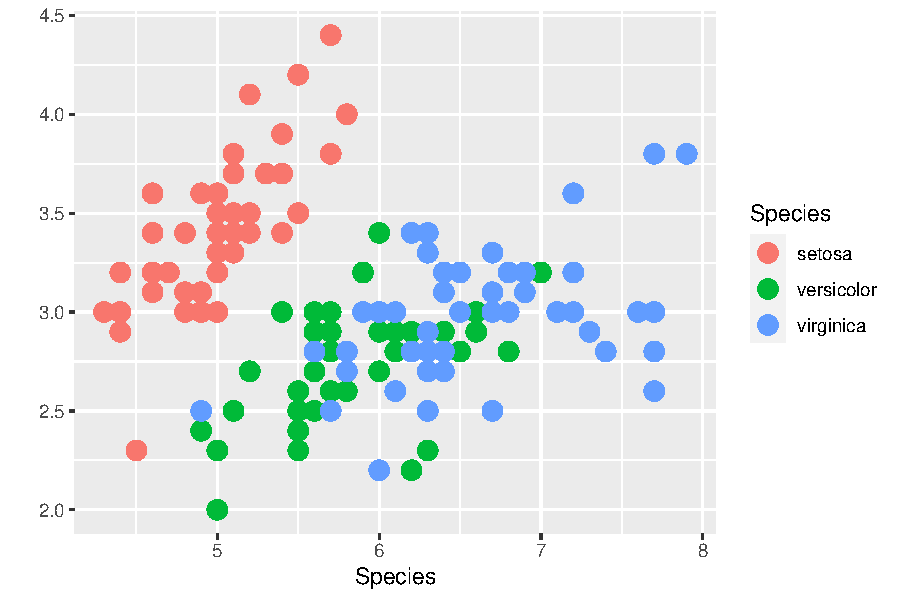
\includegraphics{using_bcggtheme_files/figure-latex/unnamed-chunk-2-1.pdf}

Finally, adjust the colours using \texttt{bcg\_colour\_manual}:

\begin{Shaded}
\begin{Highlighting}[]
\NormalTok{plot }\OperatorTok{+}
\StringTok{  }\KeywordTok{bcg_theme_classic}\NormalTok{() }\OperatorTok{+}
\StringTok{  }\KeywordTok{bcg_scale_y_continuous}\NormalTok{() }\OperatorTok{+}
\StringTok{  }\KeywordTok{bcg_colour_manual}\NormalTok{()}
\end{Highlighting}
\end{Shaded}

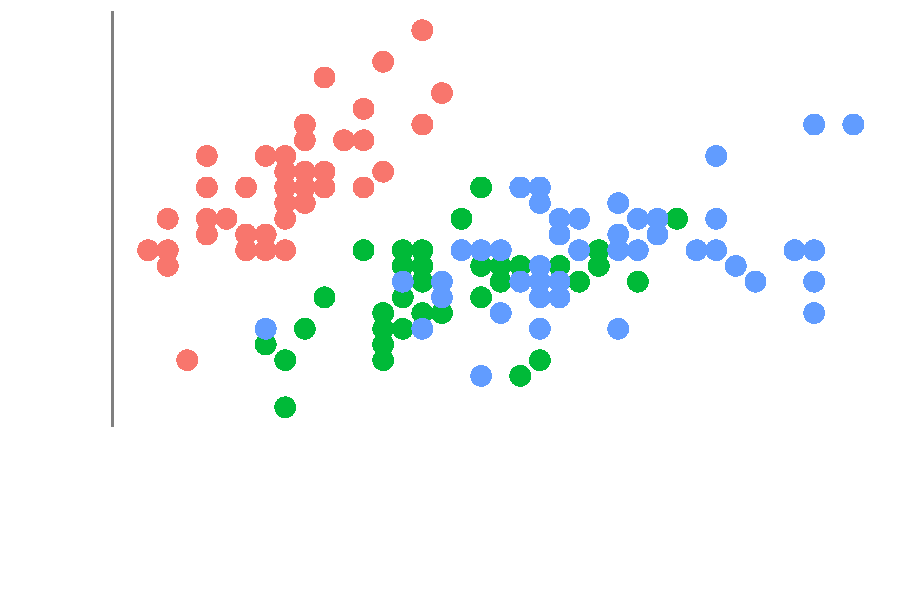
\includegraphics{using_bcggtheme_files/figure-latex/unnamed-chunk-3-1.pdf}

The standard background colour for \texttt{bcggtheme} is white. In order
to get the background the same grey colour as a BCG key message, use
\texttt{bcg\_theme\_classic(background\ =\ "grey)}

\begin{Shaded}
\begin{Highlighting}[]
\NormalTok{plot }\OperatorTok{+}
\StringTok{  }\KeywordTok{bcg_theme_classic}\NormalTok{(}\DataTypeTok{background =} \StringTok{"grey"}\NormalTok{) }\OperatorTok{+}
\StringTok{  }\KeywordTok{bcg_scale_y_continuous}\NormalTok{() }\OperatorTok{+}
\StringTok{  }\KeywordTok{bcg_colour_manual}\NormalTok{()}
\end{Highlighting}
\end{Shaded}

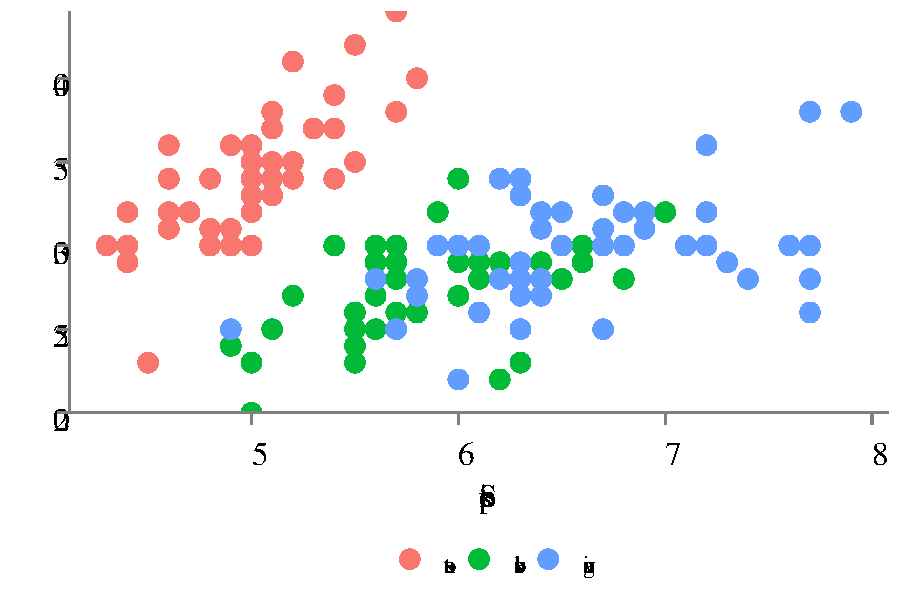
\includegraphics{using_bcggtheme_files/figure-latex/unnamed-chunk-4-1.pdf}

\hypertarget{bcg-modern}{%
\subsubsection{BCG Modern}\label{bcg-modern}}

This works best for bar charts, as will be explained later. Starting
with a made-up data set:

\begin{Shaded}
\begin{Highlighting}[]
\NormalTok{data <-}\StringTok{ }\KeywordTok{tribble}\NormalTok{(}\OperatorTok{~}\NormalTok{person, }\OperatorTok{~}\NormalTok{citations, }\OperatorTok{~}\NormalTok{school,}
                \StringTok{"Summers"}\NormalTok{, }\DecValTok{156191}\NormalTok{, }\StringTok{"Harvard"}\NormalTok{,}
                \StringTok{"Duflo"}\NormalTok{, }\DecValTok{65808}\NormalTok{, }\StringTok{"MIT"}\NormalTok{,}
                \StringTok{"Pakes"}\NormalTok{, }\DecValTok{39414}\NormalTok{, }\StringTok{"Harvard"}\NormalTok{,) }\OperatorTok\StringTok{ }
\StringTok{  }\KeywordTok{mutate}\NormalTok{(}\DataTypeTok{person =} \KeywordTok{fct_reorder}\NormalTok{(person, citations))}

\NormalTok{plot <-}\StringTok{ }\KeywordTok{ggplot}\NormalTok{(data,}
               \KeywordTok{aes}\NormalTok{(}\DataTypeTok{x =}\NormalTok{ person,}
                   \DataTypeTok{y =}\NormalTok{ citations,}
                   \DataTypeTok{fill =}\NormalTok{ school)) }\OperatorTok{+}
\StringTok{        }\KeywordTok{geom_col}\NormalTok{() }\OperatorTok{+}
\StringTok{        }\KeywordTok{labs}\NormalTok{(}\DataTypeTok{x =} \StringTok{"Economist"}\NormalTok{,}
             \DataTypeTok{y =} \StringTok{""}\NormalTok{,}
             \DataTypeTok{colour =} \StringTok{"School"}\NormalTok{)}
\end{Highlighting}
\end{Shaded}

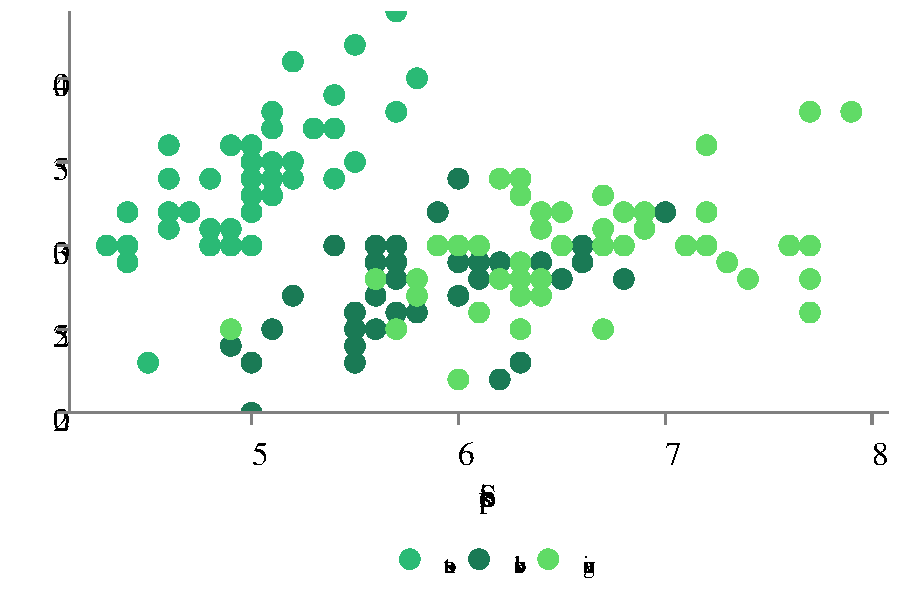
\includegraphics{using_bcggtheme_files/figure-latex/unnamed-chunk-5-1.pdf}

Then we can add the overlaying theme, using \texttt{bcg\_theme\_modern}.
The default option removes the y axis, and removes all axis tick marks

\begin{Shaded}
\begin{Highlighting}[]
\NormalTok{plot }\OperatorTok{+}
\StringTok{  }\KeywordTok{bcg_theme_modern}\NormalTok{(}\DataTypeTok{legend =} \StringTok{"right"}\NormalTok{)}
\end{Highlighting}
\end{Shaded}

\includegraphics{using_bcggtheme_files/figure-latex/unnamed-chunk-6-1.pdf}

Then we can add the other bells-and-whistles as before, noting that the
relevant colour function for is \texttt{bcg\_fill\_manual}.

\begin{Shaded}
\begin{Highlighting}[]
\NormalTok{plot }\OperatorTok{+}
\StringTok{  }\KeywordTok{bcg_theme_modern}\NormalTok{(}\DataTypeTok{legend =} \StringTok{"right"}\NormalTok{) }\OperatorTok{+}
\StringTok{  }\KeywordTok{bcg_scale_y_continuous}\NormalTok{() }\OperatorTok{+}
\StringTok{  }\KeywordTok{bcg_fill_manual}\NormalTok{()}
\end{Highlighting}
\end{Shaded}

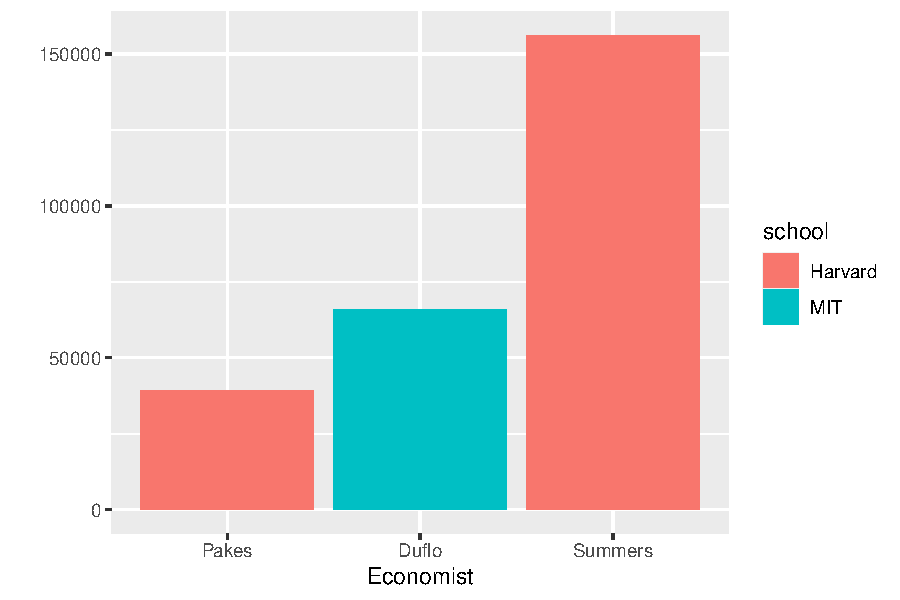
\includegraphics{using_bcggtheme_files/figure-latex/unnamed-chunk-7-1.pdf}

Clearly this chart isn't very useful, because we don't know anything
about the actual magnitude of citations for each economist. The way
around this is to add in labels. We do this using
\texttt{bcg\_geom\_label}, which adds standard grey box labels at the
top of each bar. You will then have to use \texttt{nudge\_y} to move the
box up a little bit.

\begin{Shaded}
\begin{Highlighting}[]
\NormalTok{plot }\OperatorTok{+}
\StringTok{  }\KeywordTok{bcg_theme_modern}\NormalTok{(}\DataTypeTok{legend =} \StringTok{"right"}\NormalTok{) }\OperatorTok{+}
\StringTok{  }\KeywordTok{bcg_scale_y_continuous}\NormalTok{(}\DataTypeTok{limits =} \KeywordTok{c}\NormalTok{(}\DecValTok{0}\NormalTok{,}\DecValTok{200000}\NormalTok{)) }\OperatorTok{+}
\StringTok{  }\KeywordTok{bcg_fill_manual}\NormalTok{() }\OperatorTok{+}
\StringTok{  }\KeywordTok{bcg_geom_label}\NormalTok{(}\KeywordTok{aes}\NormalTok{(}\DataTypeTok{label =}\NormalTok{ scales}\OperatorTok{::}\KeywordTok{comma}\NormalTok{(citations)), }\DataTypeTok{nudge_y =} \DecValTok{20000}\NormalTok{)}
\end{Highlighting}
\end{Shaded}

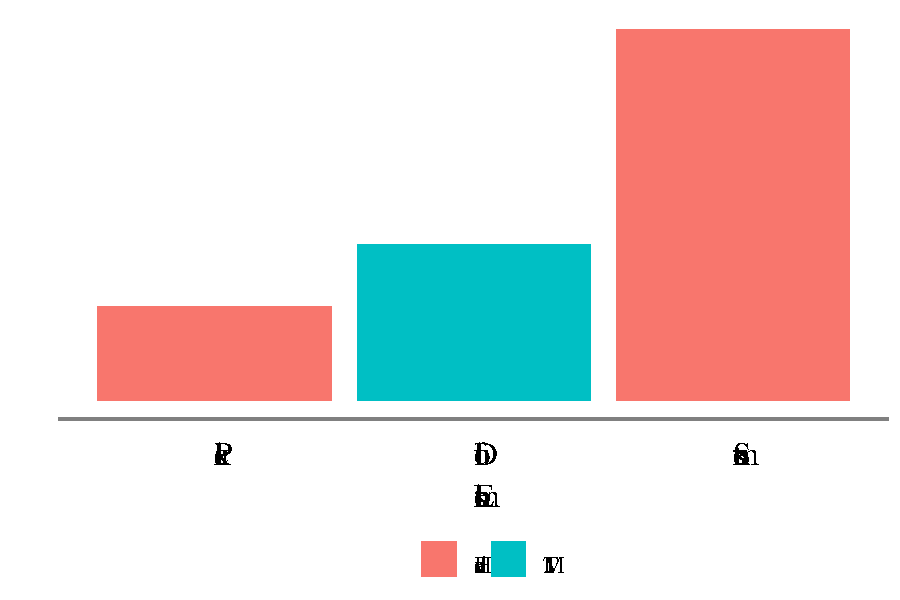
\includegraphics{using_bcggtheme_files/figure-latex/unnamed-chunk-8-1.pdf}

With the modern version we can add the y axis line back in, using
\texttt{bcg\_theme\_modern(y\_axis\ =\ TRUE)}.

\begin{Shaded}
\begin{Highlighting}[]
\NormalTok{plot }\OperatorTok{+}
\StringTok{  }\KeywordTok{bcg_theme_modern}\NormalTok{(}\DataTypeTok{legend =} \StringTok{"right"}\NormalTok{, }\DataTypeTok{y_axis =} \OtherTok{TRUE}\NormalTok{) }\OperatorTok{+}
\StringTok{  }\KeywordTok{bcg_scale_y_continuous}\NormalTok{(}\DataTypeTok{limits =} \KeywordTok{c}\NormalTok{(}\DecValTok{0}\NormalTok{,}\DecValTok{200000}\NormalTok{)) }\OperatorTok{+}
\StringTok{  }\KeywordTok{bcg_fill_manual}\NormalTok{() }\OperatorTok{+}
\StringTok{  }\KeywordTok{bcg_geom_label}\NormalTok{(}\KeywordTok{aes}\NormalTok{(}\DataTypeTok{label =}\NormalTok{ scales}\OperatorTok{::}\KeywordTok{comma}\NormalTok{(citations)), }\DataTypeTok{nudge_y =} \DecValTok{20000}\NormalTok{)}
\end{Highlighting}
\end{Shaded}

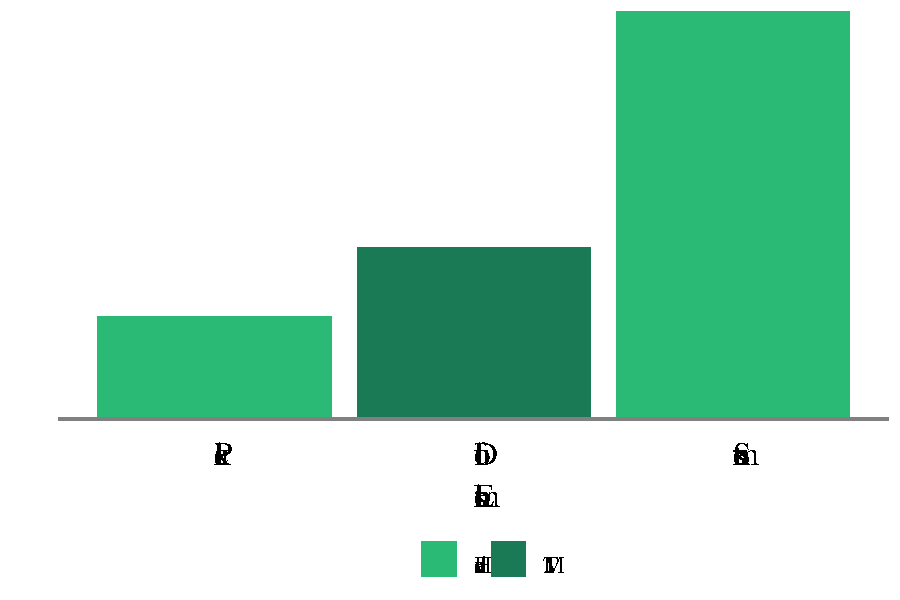
\includegraphics{using_bcggtheme_files/figure-latex/unnamed-chunk-9-1.pdf}

\hypertarget{flipped-charts}{%
\subsubsection{Flipped charts}\label{flipped-charts}}

\texttt{bcggtheme} has the function to remove the x, so that charts make
sense when used in conjunction with \texttt{coord\_flip()}.

\begin{Shaded}
\begin{Highlighting}[]
\NormalTok{plot }\OperatorTok{+}
\StringTok{  }\KeywordTok{bcg_theme_modern}\NormalTok{(}\DataTypeTok{legend =} \StringTok{"right"}\NormalTok{, }\DataTypeTok{y_axis =} \OtherTok{TRUE}\NormalTok{, }\DataTypeTok{background =} \StringTok{"grey"}\NormalTok{) }\OperatorTok{+}
\StringTok{  }\KeywordTok{bcg_scale_y_continuous}\NormalTok{(}\DataTypeTok{limits =} \KeywordTok{c}\NormalTok{(}\DecValTok{0}\NormalTok{,}\DecValTok{200000}\NormalTok{)) }\OperatorTok{+}
\StringTok{  }\KeywordTok{bcg_fill_manual}\NormalTok{() }\OperatorTok{+}
\StringTok{  }\KeywordTok{bcg_geom_label}\NormalTok{(}\KeywordTok{aes}\NormalTok{(}\DataTypeTok{label =}\NormalTok{ scales}\OperatorTok{::}\KeywordTok{comma}\NormalTok{(citations)), }\DataTypeTok{nudge_y =} \DecValTok{20000}\NormalTok{) }\OperatorTok{+}
\StringTok{  }\KeywordTok{coord_flip}\NormalTok{()}
\end{Highlighting}
\end{Shaded}

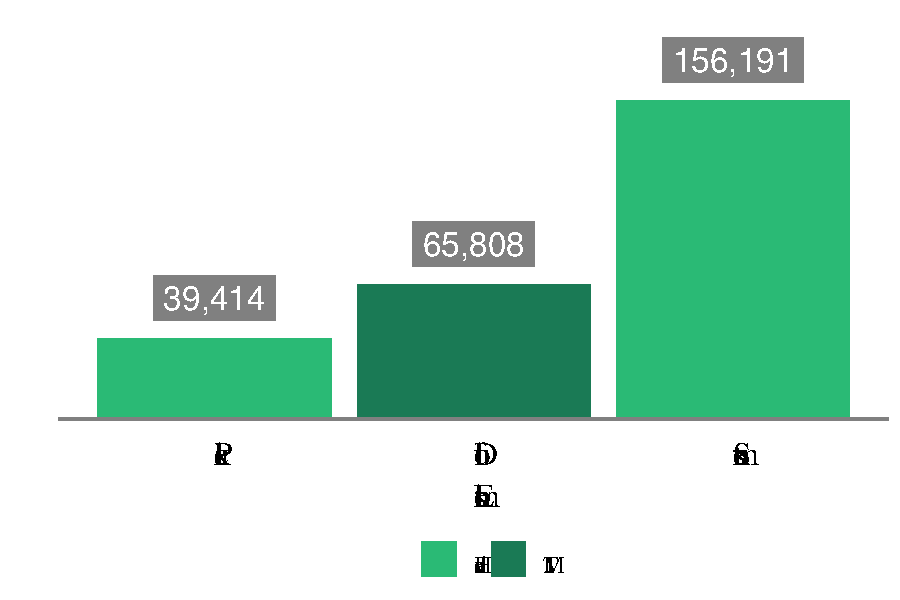
\includegraphics{using_bcggtheme_files/figure-latex/unnamed-chunk-10-1.pdf}

Then setting \texttt{bcg\_theme\_modern(flipped\ =\ TRUE)}

\begin{Shaded}
\begin{Highlighting}[]
\NormalTok{plot }\OperatorTok{+}
\StringTok{  }\KeywordTok{bcg_theme_modern}\NormalTok{(}\DataTypeTok{legend =} \StringTok{"right"}\NormalTok{,}
                   \DataTypeTok{y_axis =} \OtherTok{TRUE}\NormalTok{,}
                   \DataTypeTok{background =} \StringTok{"grey"}\NormalTok{,}
                   \DataTypeTok{flipped =} \OtherTok{TRUE}\NormalTok{) }\OperatorTok{+}
\StringTok{  }\KeywordTok{bcg_scale_y_continuous}\NormalTok{(}\DataTypeTok{limits =} \KeywordTok{c}\NormalTok{(}\DecValTok{0}\NormalTok{,}\DecValTok{200000}\NormalTok{)) }\OperatorTok{+}
\StringTok{  }\KeywordTok{bcg_fill_manual}\NormalTok{() }\OperatorTok{+}
\StringTok{  }\KeywordTok{bcg_geom_label}\NormalTok{(}\KeywordTok{aes}\NormalTok{(}\DataTypeTok{label =}\NormalTok{ scales}\OperatorTok{::}\KeywordTok{comma}\NormalTok{(citations)), }\DataTypeTok{nudge_y =} \DecValTok{20000}\NormalTok{) }\OperatorTok{+}
\StringTok{  }\KeywordTok{coord_flip}\NormalTok{()}
\end{Highlighting}
\end{Shaded}

\includegraphics{using_bcggtheme_files/figure-latex/modern_flipped-1.pdf}
Note that the same functionality applies to
\texttt{bcg\_theme\_classic()}.

\hypertarget{colours}{%
\subsubsection{Colours}\label{colours}}

The package is loaded with most standard BCG colours. Colours and
palettes are tedious to add, so it's a work in progress and some may be
missing. The colours are divided across three palettes: traffic2,
traffic3, and base (picking colours from left to right)

\begin{figure}
\centering
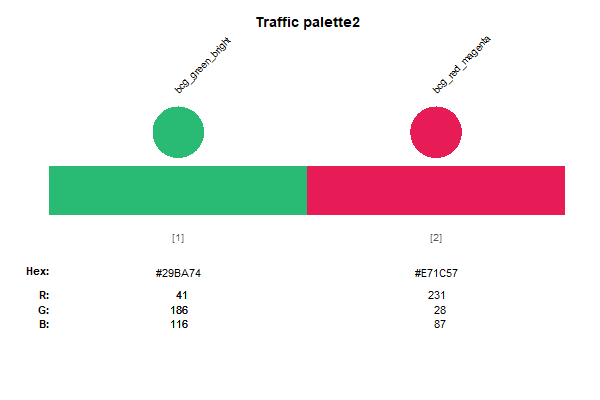
\includegraphics{traffic2.png}
\caption{Traffic palette 2}
\end{figure}

\begin{figure}
\centering
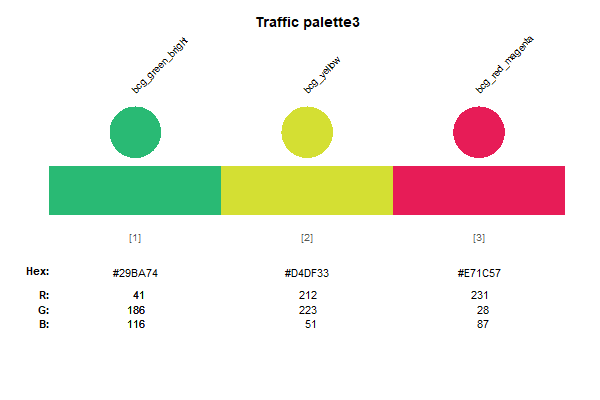
\includegraphics{traffic3.png}
\caption{Traffic palette 3}
\end{figure}

\begin{figure}
\centering
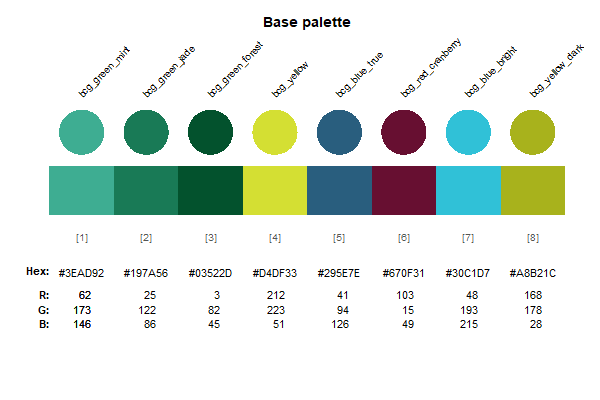
\includegraphics{base.png}
\caption{base palette}
\end{figure}

\texttt{bcg\_colour\_manual} and \texttt{bcg\_fill\_manual} can use
either palette by specifying \texttt{pal\ =\ "traffic"} or
\texttt{pal\ =\ "base"}. The colouring order can also be reversed using
the \texttt{reverse\ =\ TRUE}.

\hypertarget{outputting-charts-from-r}{%
\subsubsection{Outputting charts from
R}\label{outputting-charts-from-r}}

There are two functions to output charts: \texttt{bcg\_save} and
\texttt{bcg\_save\_pptx}. They automatically save the last object
created through ggplot.

Both output charts in up to 5 formats:

\begin{itemize}
\tightlist
\item
  ``third'': 11 cm width \(\time\) 14cm height
\item
  ``half'': 14 cm width \(\time\) 14cm height
\item
  ``two third'': 18 cm width \(\time\) 14cm height
\item
  ``large'': 24 cm width \(\time\) 14cm height
\item
  ``full'': 30 cm width \(\time\) 14cm height
\end{itemize}

These sizes are designed to replicate the options available in
ThinkCell.

\texttt{bcg\_save} and \texttt{bcg\_save\_pptx} can save any one of
these formats through \texttt{type\ =\ "chosen\ format"}. Alternatively,
all five formats can be saved by setting \texttt{type\ =\ "all"}.

For example, the following code would create a folder called
\texttt{test} within the working directory, with the relevant png charts
contained within

\begin{Shaded}
\begin{Highlighting}[]
\KeywordTok{bcg_save}\NormalTok{(}\DataTypeTok{filename =} \StringTok{"test.png"}\NormalTok{, }\DataTypeTok{type =} \StringTok{"third"}\NormalTok{) }\CommentTok{# Creates just a third slide}
\KeywordTok{bcg_save}\NormalTok{(}\DataTypeTok{filename =} \StringTok{"test.png"}\NormalTok{, }\DataTypeTok{type =} \StringTok{"all"}\NormalTok{) }\CommentTok{# Creates all five types}
\end{Highlighting}
\end{Shaded}

The following code would create a folder called \texttt{test} within the
working directory, with the relevant pptx charts contained within. The
powerpoint slides contain editable graphics, which can be easily copied
across to your desired presentation.

\begin{Shaded}
\begin{Highlighting}[]
\KeywordTok{bcg_save_pptx}\NormalTok{(}\DataTypeTok{filename =} \StringTok{"test.pptx"}\NormalTok{, }\DataTypeTok{type =} \StringTok{"half"}\NormalTok{) }\CommentTok{# Creates just a half slide}
\KeywordTok{bcg_save_pptx}\NormalTok{(}\DataTypeTok{filename =} \StringTok{"test.pptx"}\NormalTok{, }\DataTypeTok{type =} \StringTok{"all"}\NormalTok{) }\CommentTok{# Creates all five types}
\end{Highlighting}
\end{Shaded}

\texttt{bcg\_save} works best with \texttt{.png} files, currently it is
unable to output \texttt{.pdf} files. (This shouldn't be a problem. In
this line of work, I cannot imagine why you would want to directly
output to pdf).

\end{document}
